\documentclass[a4paper,12pt,twoside,openright,titlepage]{book}
\usepackage[utf8]{inputenc}
\usepackage[T1]{fontenc}
\usepackage[english]{babel}

\usepackage{amsmath}
\usepackage{amsfonts}
\usepackage{amssymb}
\usepackage{latexsym} 

\usepackage{graphicx}
\graphicspath{ {./images/} }
\usepackage{color}
\usepackage{textcomp}
\usepackage{etoolbox}    
\usepackage{listings}
\usepackage[pdftex]{hyperref}


%%% Taken from https://www.entwickler-ecke.de/topic_C+Darstellung+fuer+Latex+listings_100839,0.html

\usepackage{color}
\usepackage{listings}    
\usepackage{courier}


%%% Define Custom IDE Colors %%%
\definecolor{arduinoGreen}    {rgb} {0.17, 0.43, 0.01}
\definecolor{arduinoGrey}     {rgb} {0.47, 0.47, 0.33}
\definecolor{arduinoOrange}   {rgb} {0.8 , 0.4 , 0   }
\definecolor{arduinoBlue}     {rgb} {0.01, 0.61, 0.98}
\definecolor{arduinoDarkBlue} {rgb} {0.0 , 0.2 , 0.5 }

%%% Define Arduino Language %%%
\lstdefinelanguage{Arduino}{
  language=C++, % begin with default C++ settings 
%
%
  %%% Keyword Color Group 1 %%%  (called KEYWORD3 by arduino)
  keywordstyle=\color{arduinoGreen},   
  deletekeywords={  % remove all arduino keywords that might be in c++
break, case, override, final, continue, default, do, else, for, if, return, goto, switch, throw, try, while, setup, loop, export, not, or, and, xor, include, define, elif, else, error, if, ifdef, ifndef, pragma, warning,HIGH, LOW, INPUT, INPUT_PULLUP, OUTPUT, DEC, BIN, HEX, OCT, PI, HALF_PI, TWO_PI, LSBFIRST, MSBFIRST, CHANGE, FALLING, RISING, DEFAULT, EXTERNAL, INTERNAL, INTERNAL1V1, INTERNAL2V56, LED_BUILTIN, LED_BUILTIN_RX, LED_BUILTIN_TX, DIGITAL_MESSAGE, FIRMATA_STRING, ANALOG_MESSAGE, REPORT_DIGITAL, REPORT_ANALOG, SET_PIN_MODE, SYSTEM_RESET, SYSEX_START, auto, int8_t, int16_t, int32_t, int64_t, uint8_t, uint16_t, uint32_t, uint64_t, char16_t, char32_t, operator, enum, delete, bool, boolean, byte, char, const, false, float, double, null, NULL, int, long, new, private, protected, public, short, signed, static, volatile, String, void, true, unsigned, word, array, sizeof, dynamic_cast, typedef, const_cast, struct, static_cast, union, friend, extern, class, reinterpret_cast, register, explicit, inline, _Bool, complex, _Complex, _Imaginary, atomic_bool, atomic_char, atomic_schar, atomic_uchar, atomic_short, atomic_ushort, atomic_int, atomic_uint, atomic_long, atomic_ulong, atomic_llong, atomic_ullong, virtual, PROGMEM, Serial, Serial1, Serial2, Serial3, SerialUSB, Keyboard, Mouse,abs, acos, asin, atan, atan2, ceil, constrain, cos, degrees, exp, floor, log, map, max, min, radians, random, randomSeed, round, sin, sq, sqrt, tan, pow, bitRead, bitWrite, bitSet, bitClear, bit, highByte, lowByte, analogReference, analogRead, 
analogReadResolution, analogWrite, analogWriteResolution, 
attachInterrupt, detachInterrupt, digitalPinToInterrupt, delay, delayMicroseconds, digitalWrite, digitalRead, interrupts, millis, micros, noInterrupts, noTone, pinMode, pulseIn, pulseInLong, shiftIn, shiftOut, tone, yield, Stream, begin, end, peek, read, print, println, available, availableForWrite, flush, setTimeout, find, findUntil, parseInt, parseFloat, readBytes, readBytesUntil, readString, readStringUntil, trim, toUpperCase, toLowerCase, charAt, compareTo, concat, endsWith, startsWith, equals, equalsIgnoreCase, getBytes, indexOf, lastIndexOf, length, replace, setCharAt, substring, toCharArray, toInt, press, release, releaseAll, accept, click, move, isPressed, isAlphaNumeric, isAlpha, isAscii, isWhitespace, isControl, isDigit, isGraph, isLowerCase, isPrintable, isPunct, isSpace, isUpperCase, isHexadecimalDigit, 
                }, morekeywords={   % add arduino structures to group 1\\
  break, case, override, final, continue, default, do, else, for, if, return, goto, switch, throw, try, while, setup, loop, export, not, or, and, xor, include, define, elif, else, error, if, ifdef, ifndef, pragma, warning,}, 
% 
%
  %%% Keyword Color Group 2 %%%  (called LITERAL1 by arduino)
  keywordstyle=[2]\color{arduinoBlue},   
  keywords=[2]{   % add variables and dataTypes as 2nd group  
HIGH, LOW, INPUT, INPUT_PULLUP, OUTPUT, DEC, BIN, HEX, OCT, PI, HALF_PI, TWO_PI, LSBFIRST, MSBFIRST, CHANGE, FALLING, RISING, DEFAULT, EXTERNAL, INTERNAL, INTERNAL1V1, INTERNAL2V56, LED_BUILTIN, LED_BUILTIN_RX, LED_BUILTIN_TX, DIGITAL_MESSAGE, FIRMATA_STRING, ANALOG_MESSAGE, REPORT_DIGITAL, REPORT_ANALOG, SET_PIN_MODE, SYSTEM_RESET, SYSEX_START, auto, int8_t, int16_t, int32_t, int64_t, uint8_t, uint16_t, uint32_t, uint64_t, char16_t, char32_t, operator, enum, delete, bool, boolean, byte, char, const, false, float, double, null, NULL, int, long, new, private, protected, public, short, signed, static, volatile, String, void, true, unsigned, word, array, sizeof, dynamic_cast, typedef, const_cast, struct, static_cast, union, friend, extern, class, reinterpret_cast, register, explicit, inline, _Bool, complex, _Complex, _Imaginary, atomic_bool, atomic_char, atomic_schar, atomic_uchar, atomic_short, atomic_ushort, atomic_int, atomic_uint, atomic_long, atomic_ulong, atomic_llong, atomic_ullong, virtual, PROGMEM,},  
% 
%
  %%% Keyword Color Group 3 %%%  (called KEYWORD1 by arduino)
  keywordstyle=[3]\bfseries\color{arduinoOrange},
  keywords=[3]{  % add built-in functions as a 3rd group
                Serial, Serial1, Serial2, Serial3, SerialUSB, Keyboard, Mouse,
                },      
%
%
  %%% Keyword Color Group 4 %%%  (called KEYWORD2 by arduino)
  keywordstyle=[4]\color{arduinoOrange},
  keywords=[4]{  % add more built-in functions as a 4th group
abs, acos, asin, atan, atan2, ceil, constrain, cos, degrees, exp, floor, log, map, max, min, radians, random, randomSeed, round, sin, sq, sqrt, tan, pow, bitRead, bitWrite, bitSet, bitClear, bit, highByte, lowByte, analogReference, analogRead, 
analogReadResolution, analogWrite, analogWriteResolution, 
attachInterrupt, detachInterrupt, digitalPinToInterrupt, delay, delayMicroseconds, digitalWrite, digitalRead, interrupts, millis, micros, noInterrupts, noTone, pinMode, pulseIn, pulseInLong, shiftIn, shiftOut, tone, yield, Stream, begin, end, peek, read, print, println, available, availableForWrite, flush, setTimeout, find, findUntil, parseInt, parseFloat, readBytes, readBytesUntil, readString, readStringUntil, trim, toUpperCase, toLowerCase, charAt, compareTo, concat, endsWith, startsWith, equals, equalsIgnoreCase, getBytes, indexOf, lastIndexOf, length, replace, setCharAt, substring, toCharArray, toInt, press, release, releaseAll, accept, click, move, isPressed, isAlphaNumeric, isAlpha, isAscii, isWhitespace, isControl, isDigit, isGraph, isLowerCase, isPrintable, isPunct,isSpace, isUpperCase, isHexadecimalDigit,},      
%
%
  %%% Set Other Colors %%%
  stringstyle=\color{arduinoDarkBlue},    
  commentstyle=\color{arduinoGrey},    
%          
%   
  %%%% Line Numbering %%%%
   numbers=left,                    
  numbersep=5pt,                   
  numberstyle=\color{arduinoGrey},    
  %stepnumber=2,                      % show every 2 line numbers
%
%
  %%%% Code Box Style %%%%
  breaklines=true,                    % wordwrapping
  tabsize=2,         
  basicstyle=\ttfamily  
}
\usepackage{courier, color, listings}

\definecolor{Green}{rgb}{0, 0.3, 0}
\definecolor{DarkCyan}{rgb}{0, 0.545, 0.545}
\definecolor{Navy}{rgb}{0, 0, 0.5}
\definecolor{Teal}{rgb}{0, 0.5, 0.5}
\definecolor{DarkGray}{gray}{0.66}
\definecolor{Olive}{rgb}{0.5, 0.5, 0}
\definecolor{Pink}{rgb}{1.0, 0.75, 0.8}
\definecolor{DeepPink}{rgb}{1, 0.08, 0.58}
\definecolor{Brown}{rgb}{0.65, 0.165, 0.165}
\definecolor{DarkViolet}{rgb}{0.58, 0, 0.83}
\definecolor{SaddleBrown}{rgb}{0.55, 0.27, 0.07}
\lstdefinelanguage{CSharp}
{
 morecomment = [l]{//}, 
 morecomment = [l]{///},
 morecomment = [s]{/*}{*/},
 morestring=[b]", 
 morestring=[b]',
 basicstyle=\footnotesize\ttfamily,
 commentstyle=\color{Green}\textit,
 stringstyle=\color{blue},
 sensitive = true,
  morekeywords=[1]{this, base},
  keywordstyle=[1]\bfseries,
  morekeywords=[2]{as, is, new, sizeof, typeof, true, false, stackalloc, ArduinoData, Key},
  keywordstyle=[2]\color{DarkCyan}\bfseries,
  morekeywords=[3]{else, if, switch, case, default,
  do, for, foreach, while, in},
  keywordstyle=[3]\color{blue}\bfseries ,
  morekeywords=[4]{break, continue, goto, return,
  yield, partial, global, where},
  keywordstyle=[4]\color{Navy},
  morekeywords=[5]{try, throw, catch, finally},
  keywordstyle=[5]\color{Teal}\bfseries,
  morekeywords=[6]{checked, unchecked},
  keywordstyle=[6]\color{DarkGray}\bfseries,
  morekeywords=[7]{fixed, unsafe},
  keywordstyle=[7]\color{Olive},
  morekeywords=[8]{bool, byte, sbyte, char, short, ushort, int, uint, long, ulong, float,
  double, decimal, enum, struct},
  keywordstyle=[8]\bfseries\color{blue},
  morekeywords=[9]{class, interface, delegate, object, string,
  void},
  keywordstyle=[9]\color{red},
  morekeywords=[10]{explicit, implicit, operator},
  keywordstyle=[10]\color{Pink}\bfseries,
  morekeywords=[11]{params, ref, out},
  keywordstyle=[11]\bfseries\color{DeepPink},
  morekeywords=[12]{private, protected, internal, public},
  keywordstyle=[12]\bfseries\color{blue},
  morekeywords=[13]{abstract, const, event, var, override, virtual, volatile, extern, readonly, sealed, static},
  keywordstyle=[13]\color{Brown},
  morekeywords=[14]{namespace, using},
  keywordstyle=[14]\bfseries\color{Green},
  morekeywords=[15]{lock},
  keywordstyle=[15]\color{DarkViolet},
  morekeywords=[16]{get, set, add, remove},
  keywordstyle=[16]\color{SaddleBrown},
  morekeywords=[17]{null, value},
  keywordstyle=[17]\bfseries,
}
\lstset{tabsize=4,showstringspaces=false, numberstyle=\tiny, stepnumber=2, numbersep=5pt}
\newenvironment{dedication}%
{\cleardoublepage\addcontentsline{toc}{chapter}{Dedication}\null\vfill\begin{flushright}}%
{\end{flushright}\vfill\null}


\newenvironment{abstract}%
{\cleardoublepage\addcontentsline{toc}{chapter}{Abstract}\null\vfill\begin{center}%
\bfseries\abstractname\end{center}}%
{\vfill\null}

\title{Automatic Gardening System}
\author{Kristmund Ryggstein and Hergeir Winther Lognberg \\ University of the Faroe Islands\\}


\begin{document}
\frontmatter
\maketitle

\frontmatter
\maketitle

\begin{abstract}
We were asked to do an it project using an Arduino Uno. We chose to to do an automated gardening system with it, because that is relevant for some work projects that are currently in progress on Sandoy, where we are from. Our ardunio project entails an automated system that waters, measures moisture, heat and light exposure. That is done by customizing an Arduino Uno which has a moisture-, heat and light sensor that does all our measurements. All the the data is then collected by the Arduino, and then sent to a Web Service via. a esp-05 wifi module. The Web Service receives the data, and presents it to the user. The user is registered with the Web Service, and can track his plant data through his registered user account, where he also can customize water input for the plant/s.
\end{abstract}

\cleardoublepage\addcontentsline{toc}{chapter}{Contents}
\tableofcontents

\chapter{Foreword}

The foreword often consists of the author's personal opinion, the history of how the work emerged, how the work is structured, how the reader can choose to read it etc. It might also contain dedications, acknowledgements and similar things. 

\section*{Acknowledgement}
We want to thank The University of The Faroe Islands for providing us with the materials provided to us from the beginning, and to thank them for providing us with the funds to procure new materials. We also want to thank Benadikt Joensen for guiding  and teaching us on the more electrical side of things in our project.
\addcontentsline{toc}{section}{Acknowledgement}

\mainmatter
\chapter{Introduction}

The purpose of this report is to document our project and the process of developing it.

We have chosen to work with automatic a gardening system because it has some tasks, what we believe, are tedious and easy to forget. There has been an increasing interest on Sandoy in trying to grow more vegetables on the islands, and to sell them. That grown interest in thanks to initiatives such as "Veltan" and "Eplafestivalurin". Trying to be self-sufficient with regards to food produce is, according us, a good idea, and that's were we think that our modest electronic gardening project fits well with that philosophy, and will be an interest for those, who want to try to be more self-sufficient.
 
\addcontentsline{toc}{section}{Introduction}

\chapter{Setup}
The Arduino Uno, TMP36GZ heat sensor, resistors and the cables which we use in this project, was provided by the one responsible by the course. We used at the start a FC28 moisture sensor, but it generally uses DC current which means that it corrodes quickly because of electrolysis in the soil and alters the soil composition which could potentially damage the plant. That would also eventually lead to tainted readings. We changed it to use an AC pulse that can be seen in figure, but we decided to opt for Capacitive Soil Moisture Sensor V1.2 that is Corrosion Resistant. The FC28 sensor can be seen in \ref{fig:resistive} and the Capacitive sensor can be seen in figure \ref{fig:capacitive}.

\section{Arduino}
Arduino is an open-source electronics platforms which is based on user-friendly software and hardware components\cite{ArduinoIntroduction}. It can read outputs from these components e.g. readings from sensors, and it can give input to these sensors.

We worked on an Arduino Uno. It is a microcontroller board. It has 14 digital i/o pins. they can be located on the board right next to the text \textit{DIGITAL}. Six of those pins can be used as Power Width Modulation, shortened as PWM, outputs. Those pins are the ones who have a ~ next to their ascribed numbers. It has six analog pins. It then has five different kinds of power pins. We only use the GND and the 5V and 3.3V pins. The 5V and 3.3 pins output a 5V and 3.3V from the regulator on the board which can be used to power different hardware components. The 3.3V pins has a maximum current draw of 50mA. GND stands for ground, and serves as the common return path for current from the different hardware components in our Arduino system. 

\section{Moisture Sensors}
\subsection{FC28}
Our intention was to use the Arduino to induce an alternating current through the sensor. To simplify things, we circumvented the circuit of FC-28 such that we connected directly to the pins on the sensor. To alternate the current, we first emit 5V from pin 12 and set pin 13 to low (0V) for 1 ms then we take a reading through the analog pin A0. Then we flip the pin 12 and 13 ( 5V from pin 13 ) for the same amount of time. This should somewhat remedy the problems of electrolysis by shifting the ions back and forth between the moisture sensor pins, instead of just letting them congest at one pin. The chip had to be removed so that it could use AC.
The setup can be seen below.


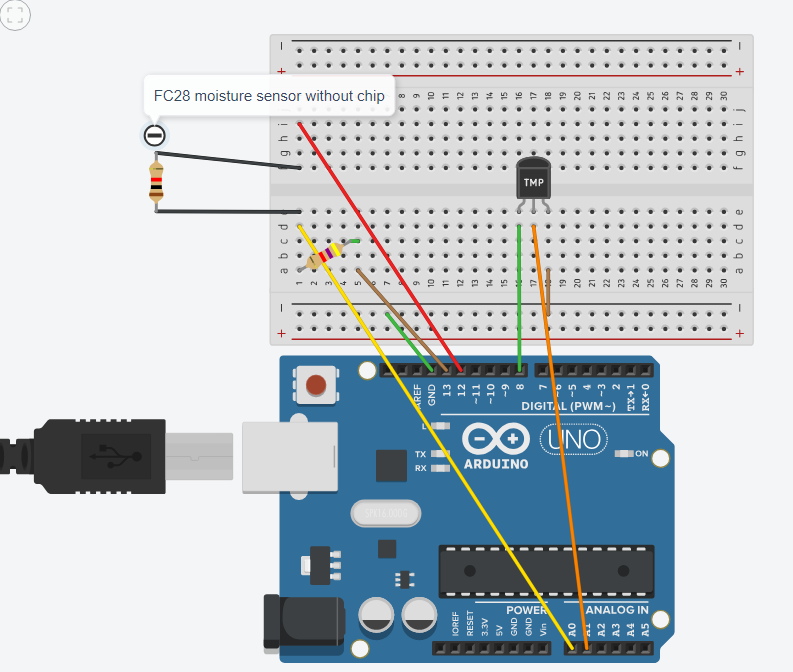
\includegraphics[scale = 0.50]{FC-28-Diagram.PNG}

The resistor in the circuit helps increase the amount of current entering the analog sensor. Without it about half the current would go in the pin 13 when the measurement occurs. We are therefor able to steer the range of current entering the analog input. The left left leg is connected to 8 digital pin, the middle leg is connected to A1 pin, and the third leg is connected to -18 on the breadboard which is then connected to the ground pin on the Arduino.  

\subsection{Capacitive Soil Moisture Sensor v1.2}
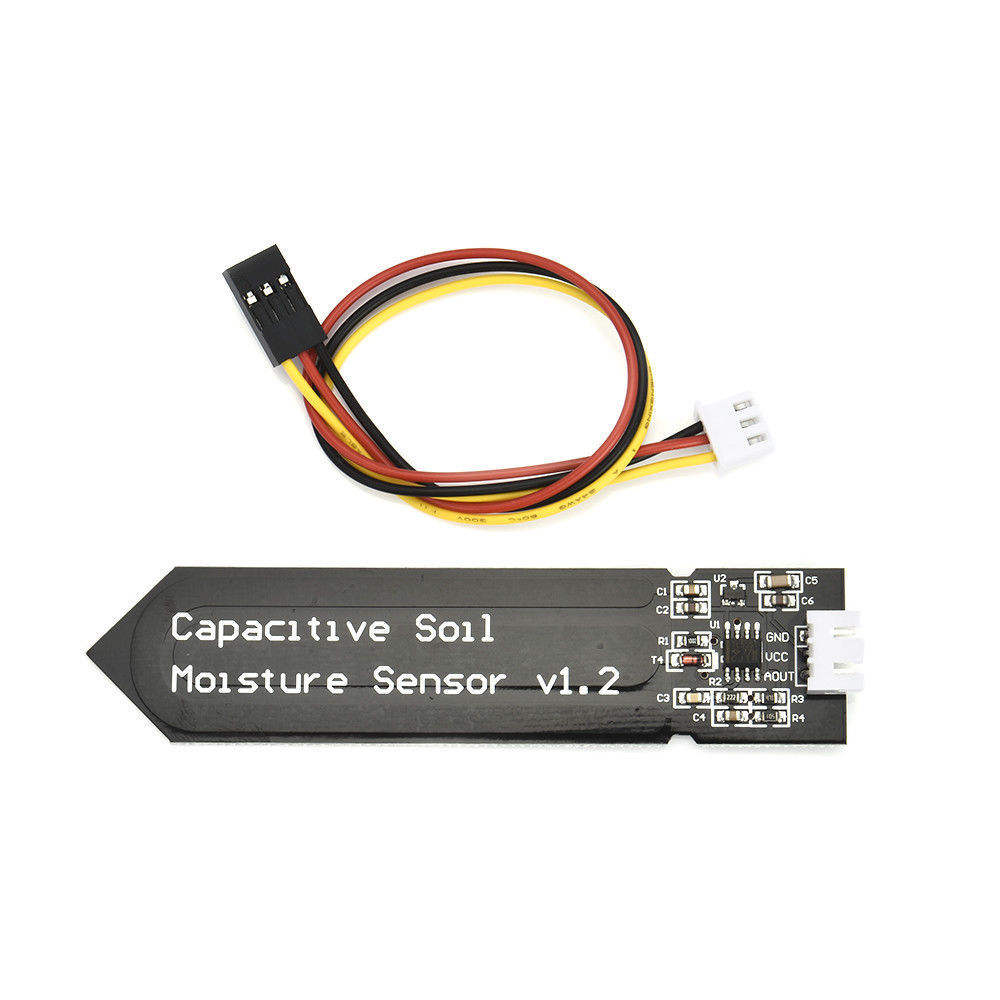
\includegraphics[scale=0.40]{capacitive-sensor}

We looked at reviews, and this one seemed to be the most corrosion resistant of the ones we looked at. It is made by corrosion resistant material, so it has a higher lifetime than the other sensor. It measures moisture, or rather the ions in the soil, by reading the capacitance between two plates in the sensor. It has lesser range than the other one, as it measures air values as 555 and completely submerges as 280. We thought the minimized range wouldn't worsen our readings, and the benefit from increased lifetime far outweighed it.

\begin{lstlisting}[language=Arduino]
uint8_t CapacitiveMoistureSensor::readPercent(uint16_t val)
{
     /* 555 is the value for moisture in the air
	 // 288 is the value for when the sensor is submerged in water
	  then sett 555 to be 0%, 288 to be 100%, and map the percent between them */
	
	val = constrain(val,280,555);
	double valPercent = map (val, 555, 280, 0, 100);

	return valPercent;
}

\end{lstlisting}
readPercent takes the read value from the analog read, and converts it to a percent that is mapped between air- and water value. Line 7 sets a constrain on val variable which says that it can't be more than 55 and not less than 280. Line 8 creates a new variable, which is val parameter mapped as a percentage between 555 and 280 where 555 is 0\% and 280 is 100\%.

\begin{lstlisting}[language=Arduino]
uint8_t CapacitiveMoistureSensor::read()
{
	digitalWrite(dPin,HIGH);
	delay(1000);
    uint16_t val = analogRead(aPin);
	
    return readPercent(val);
}
\end{lstlisting}

This method reads the output from the capacitive sensor. digitalWrite(dPin, HIGH) starts the sensor. dPin is the the digital pin in which the sensor is connected to the Arduino. delay(1000) pauses the code at one second, then it initalized the val varaiable through analogRad(aPin), where aPin is the analog pin which the sensor is connected. Then the method calls and  the above readPercent(val) method, which converts the value to a percentage, and the read() method returns that percentage to where the method was called from i.e. the main Arduino program.

\section{Temperature Sensor}
\subsection{TMP Sensor}
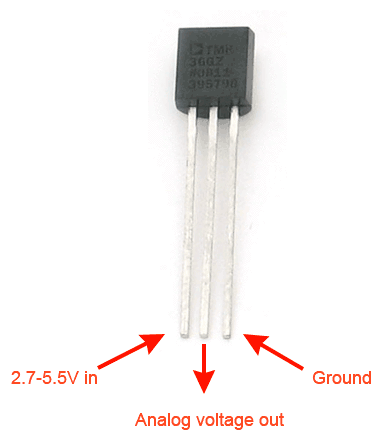
\includegraphics[scale=1]{TMP-36}

We used the TMP36 temperature sensor, as it was supplied to use by the course administrators and that it suits our purpose. The TMP36 is fairly simple. It can measure degrees from -40\textdegree{}C to \textdegree{125}C, where it has a precision\cite{tmpTutorial} of $\pm2$\textdegree{}C. It works as a diode so when it changes temperature, it then its voltage changes accordingly. The sensor measures the small change and outputs an analog output based on it, so its possible to calculate the temperature according to that output. 
The sensor's collector pin is attached to the 8 digital pin, the gate to the analog input A1 and the third leg is 
We use a readCelcius() method from the Temperature Class, and it can be seen below.
\begin{lstlisting}[language=Arduino]
const int8_t TemperatureSensor::readCelsius()
{
    digitalWrite(triggerPin, HIGH);
    delayMicroseconds(200);
    uint16_t reading = analogRead(readPin);
    digitalWrite(triggerPin, LOW);
    // converting that reading to voltage, for 3.3v arduino use 3.3
    double voltage = reading * 5.0; // * 0.0009775171;
    voltage /= 1024.0;
    return round((voltage - 0.5) * 100);
}
\end{lstlisting}
digitalWrite(triggerPin, HIGH) sends a pulse to the sensor which starts it, then delayMicroseconds() delays the program, so that the sensor waits while the sensor is activated. Then reading = analogRead(readPind) reads the output from the sensor. The output from it, is converted to voltage by multiplying it with five. That is then divided by 1024 to find the percentage of the analog read, because the Arduino outputs between 0 and 1023, where 0 is not voltage and 1023 is 5V. Five is then subtracted from that, and then that result is multiplied with 100 to convert it from mV to degrees. Five is subtracted from the reading because we want it so that 0V corresponds to -50\textdegree{}C. 

\section{Light Sensor}
\subsection{LDR Resistor}
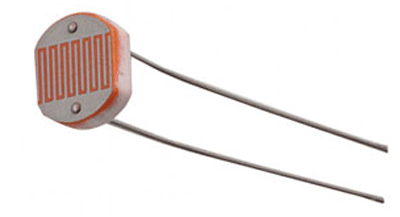
\includegraphics[scale=0.80]{LDR-Resistor}

We use a LDR Resistor to detects the level of light in the room. The resistor changes its resistance based on how much light is in the room. If the room is unlit then the resistor will have a resistance of a few ohms, but will decrease if the room gets lighter. It's not ideal for our purpose because it's not very sensitive, and that it needed to be calibrated. We chose it because it was available and that we wanted to focus on the webserver and other areas of the project.

\section{Water Pump}
\begin{center}
	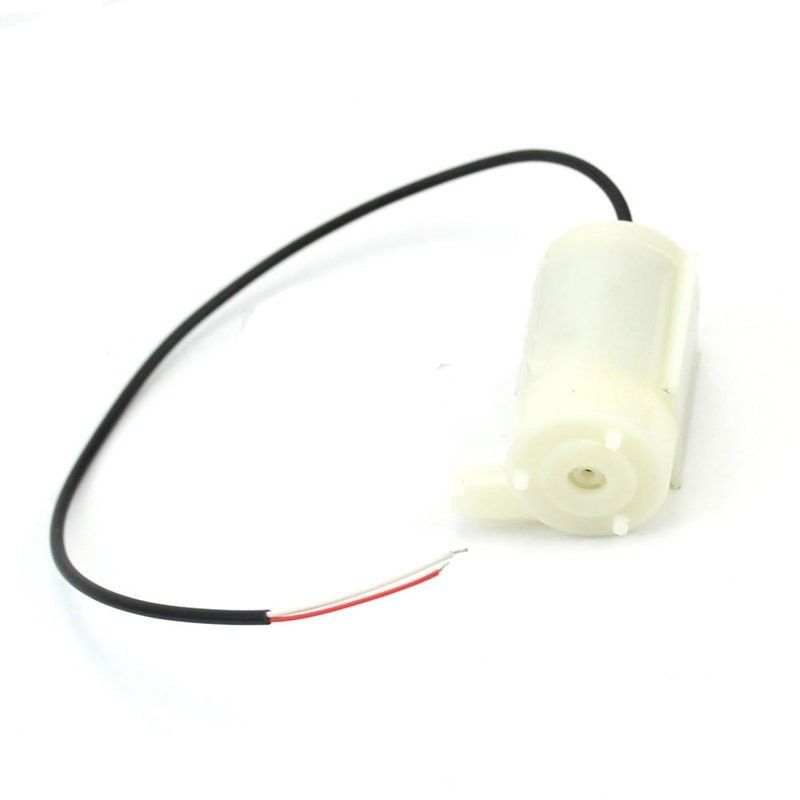
\includegraphics[scale=0.3]{Water-Pump}
\end{center}

Our water pump is said to have a flow rate of 80-120L\\H. We haven't tested that, but our tests deem that it is strong enough for our purpose- maybe even too strong. It uses a DC current 2.5-6V. The rest of the product description is in \ref{fig:pump description}. Its tube was bought in the local Pet store, and was glued on the facing  left in the picture.

\section{Wifi Module}
\begin{center}
	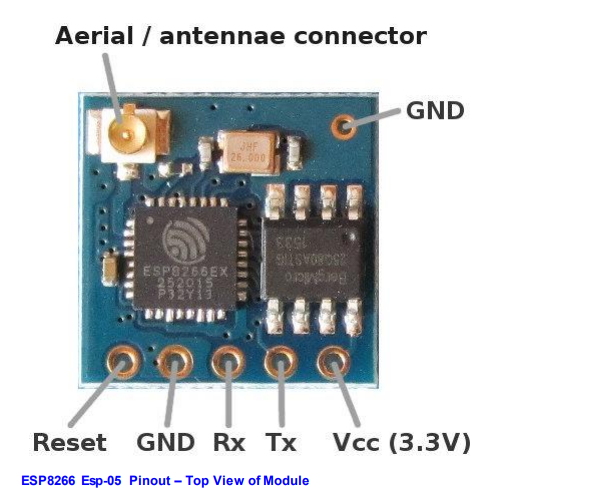
\includegraphics[scale=0.3]{ESP8266}
\end{center}

The ESP8266-05 wifi module was the hardest to work with. We initially bought an ESP8266-01\ref{fig:ESP}, but that was even tougher to work with, because it had 8 pins, and the distance between each pin on the module was so small that we couldn't properly solder each part without connecting it to the next one. We then bought the 05 version which was much easier to solder. A picture is attached of the module in \ref{fig:ESP}. We don't use the antennae nor the upper GND pin. We have a problem with the module in that the Arduino UNO 3V supply has inadequate current capabilities to power it. It still works but we get occasional garbage data from the packages sent sent from the module. Garbage transmissions seem to increase the longer the module is in use. It's possible to use an alternate 3.3V supply rather than the one from the Arduino but we didn't look into it, as it would take focus from some of the other work needed in the development.

\chapter{Website}
\section*{Webserver}
We chose to work with Microsoft's ASP.NET Core which is an open-source cross-platform framework for building cloud-based and internet-connected applications. We chose this framework because we familiar with it through the course 5022.16 Web Applications: ASP.NET with C\# which we had right before this course. It is something both collaborators in this project like to use. 


\section{Hosting}
We initially chose to host the webserver on Microsoft's Azure, which all university students get access to through Microsoft's student offer. We quickly found out that it didn't work for us, because it only allows port 8080 and port 443 to be open. We needed other ports to use for communicating between the Arduino and the webserver.

\section{Login}
We found out that .Net Core has something called Identity Core\cite{Identity} which handles the login for an ASP.NET Core application. The user can create a membership for the application by using his or she's  Facebook, Twitter, Microsoft, or Google login credentials. We could have added the other options, but we deemed it unnecessary as most faroese that would be willing to use a system such ours will most likely have a Facebook account. It's also possible to login with a regular email.

\begin{lstlisting}, language=CSharp] 
services.AddAuthentication().AddFacebook(facebookOptions =>
{
	facebookOptions.AppId =
			 Configuration["Authentication:Facebook:AppId"];
	facebookOptions.AppSecret =
			 Configuration["Authentication:Facebook:AppSecret"];
});
\end{lstlisting}
This code block adds Facebook authentication to our login service. facebookOptions.AppId and facebookOptions.AppSecret are plugins from chrome, which had to be created in Chrome to support facebook login for our project. We found the tutorial for it on \href{https://docs.microsoft.com/en-us/aspnet/core/security/authentication/social/facebook-logins?view=aspnetcore-2.2}{Microsoft's support page for identity on}. The idea with the login functionality is that plants can be attached to users in our system, and that he is able to view data about his plants on the website.


\subsection{Project E.Garden Structure}
Our .Net Core project is divided into three parts. It's good practice to have all business logic i.e. models that represents plants, users, and Arduino Data in a separate class library from the main program. It's done so the project is decoupled, and so that the classes can be included in a separate project. This class library is called Repository in our project, and structure of it is also divided into three parts. First part is the Model folder where the classes are and can be seen in \ref{list:Models}. ApplicationUser inherits from User, because that makes it so that the properties from ApplicationUser gets added to AspNetUsers in the database. That is a functionality of the previously mentioned Identity. 

One part of the library is a folder that contains the skeleton i.e. interfaces for our business handling, then the implementation of those interfaces is located in the Concrete folder. This means that the EFPlantRepository model inherits from IPlantRepository, and then specifies what the methods UserPlants() and SavePlants() should do. These repositories are then initialized in the file Startup.cs, specifically the ConfigureServices(IServiceCollection services) method. It's initialized with something called Dependency Injection\href{https://docs.microsoft.com/en-us/aspnet/core/fundamentals/dependency-injection?view=aspnetcore-2.2}, and that can be seen in below.

\begin{lstlisting}[caption={Dependency Injection}\label{list:DpInjection}, language=CSharp]
	services.AddScoped<IApplicationUserAccessor, ApplicationUserAccessor>();
	services.AddScoped<IPlantRepository, EFPlantRepository>();
    services.AddScoped<IArduinoDataRepository, EFArduinoDataRepository>();
\end{lstlisting}

This initializes at run time all instances of those three interfaces in the project as the EF implementation to the right of them. AddScoped or AddTransient establishes the lifetime of the services, and scoped means that it is created once per request. The code for the interfaces can be seen in \ref{list:Interface Repositories}. The implementations and the explanations for the interfaces can be seen below.

\begin{lstlisting}[caption={Observer Class}\label{list:Concrete EFArduinoDataRepository}, language=CSharp]
public class EFArduinoDataRepository : IArduinoDataRepository
{
	private readonly EGardenerContext _context;
        
	public EFArduinoDataRepository(EGardenerContext context)
	{
        _context = context;
	}
	public void SaveData(ArduinoData data)
	{
		var context = _context;
		var plants = context.Plants.Include(x => x.Datas);
	    var plant = plants.Single(x => x.PlantId == data.PlantId);
        var datas = plant.Datas;
        datas.Add(data);
		context.SaveChanges();
	}

}
\end{lstlisting}

It has one private datamember called \_context of type EGardenerContext, which gets initialized in the EFArduinoDataRepository. This context is the context between the models and their corresponding database entities. All the EFRepositories have this EGardenerContext. The SaveData(Arduino Data) is the actual implementation of the IArduinoDataReposistory. It takes an ArduinoData object as a parameter. First a new context variable is initializied, then a plant gets initialized by dotting into the context, and choosing a plant in the database that has a PlantId that corresponds to plantId the data parameter has. A list of data gets initialized by assigning it to the data list in the newly created plant, and then the data parameter is added to that list. context.SaveChanges(); saves all the changes made.  


\begin{lstlisting}[caption={Observer Class}\label{list:Concrete EFPlantRepository}, language=CSharp]
public class EFPlantRepository : IPlantRepository
{
	private readonly EGardenerContext _context;
    private readonly IApplicationUserAccessor _userAccessor;

	public EFPlantRepository(EGardenerContext context,
	IApplicationUserAccessoruserAccessor)
	{
		_context = context;
        _userAccessor = userAccessor;
	}

        
	public async Task<IEnumerable<Plant>> UserPlants()
	{

		var user = await _userAccessor.User;
            
		user = _context.Users.Include(x => x.Plants)
			.ThenInclude(x => x.Datas).Single(x => x.Id == user.Id);
            
            return user?.Plants ?? new List<Plant>();
	}

	public async Task SavePlant(Plant plant)
	{
		var user = await _userAccessor.User;
		var dbUser = await _context.Users.FindAsync(user.Id);

		plant.ApplicationUser = user;
		if (dbUser.Plants == null)
		{
	        dbUser.Plants = new List<Plant>();
        }
            
        dbUser.Plants.Add(plant);
        var amount = await _context.SaveChangesAsync();
	}
}
\end{lstlisting}
This class has a private field of type IApplicationUserAccessor called userAccessor which is used to access the users in the database. UserPlants() returns an asynchronous task that takes an IEnumerable<Plant>. IEnerumable is a C\#  build in interface which makes it easy to work with any kind of containers. var user = await userAccessor.User initializes the variable with user that is currently logged in. Await means that the method has to wait that initialization to finish in order to continue. User is then reassigned to the entity in the database that shares the same Id. Include(x => x.Plants) includes the plant list from the database user. ThenInclude then includes datas to each plant in the previous list. Single(x => x.Id == user.Id) finds the correct user. The method then either returns the user's plants or returns a new plant list. It returns the user plants when the user is not null and plants is also not null.

SavePlant(Plant pltant) is an asynchronous method that stores a plant in the database.  It also initializes a user with the HttpContext, but it also creates one dbUser with one from the database. The dbUser is initialized similarly with how the user in UserPlants() got reassigned, and that is by locating it by user Id. The method suspends when it initialized those variables. The parameter, plant, then initializes its own user property to the user in this method. If db.User has an uninitalized plants property, then it gets initalized with a new empty one. The plant parameter then gets added to that plants property, and the \_context asynchronously saves the changes.  
\subsection{Observer Pattern}
We decided to use \href{https://en.wikipedia.org/wiki/Observer_pattern}{Gang Of Four's observer pattern}. We think that it fit well in our implementation of the communication between the Arduino and our Webserver. Microsoft have their own implementation of the pattern\href{https://docs.microsoft.com/en-us/dotnet/standard/events/observer-design-pattern}{pattern}
 
In short, the pattern is about having one subject that has a list of dependencies which it notifies when there's a change.

\subsubsection{Observer}
Our provider is called Observer and implements the IObserver with ArduinoData in the template brackets. That it implements the interface means that the class implements its own version of the methods
\begin{itemize}
\item OnCompletet()
\item OnError(Exception Error)
\item OnNext(T Value)
\end{itemize}

These can be called event handlers as they get called, when those events happen. The first method indicates that the provider is finished with transferring data. Second method informs the observer that an error occurred. The third method supplies the observer with current or new data. 
The class has one member variable called \_unsubscriber, which is an IDisposable object, and it has two properties of type ArduinoData called Data and type String which is the Observer's name. IDisposable is a C\# interface that provides a mechanism for releasing unmanaged resources by its method Dispose(). ArduinoData is one we made, and it is the container for the data in which the arduino transfers to the webserver. It's properties can be seen in listings \ref{lst:ArduinoDataRepository}

\subsubsection{Observable}

\appendix

\chapter{Graphics of sensors and other components}
The following are pictures of our sensors and other components.

\begin{figure}[!ht]
  \centering
      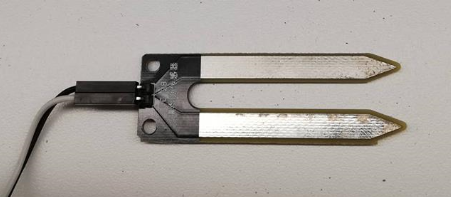
\includegraphics{fc-28-corrosion}
  \caption{Corroded fc-28 after moderate use.}
  \label{fig:resistive}
\end{figure}

\begin{figure}[ht!]
	\begin{itemize}
	\item 100\% brand new and high quality
	\item DC Voltage:2.5-6V
	\item Maximum lift:40-110cm / 15.75"-43.4"
	\item Flow rate:80-120L/H
	\item Outside diameter of water outlet: 7.5mm / 0.3"
	\item Inside diameter of water outlet: 4.7mm / 0.18"
	\item Diameter:Approx. 24mm / 0.95"
	\item Length:Approx. 45mm / 1.8"
	\item Height:Approx. 33mm / 1.30"
	\item Material:engineering plastic
	\item Driving mode: brushless dc design, magnetic driving
	\item Continuous working life of 500 hours
	\end{itemize}
	\label{fig:pump description}
\end{figure}


\begin{figure}[!ht]
	\centering
		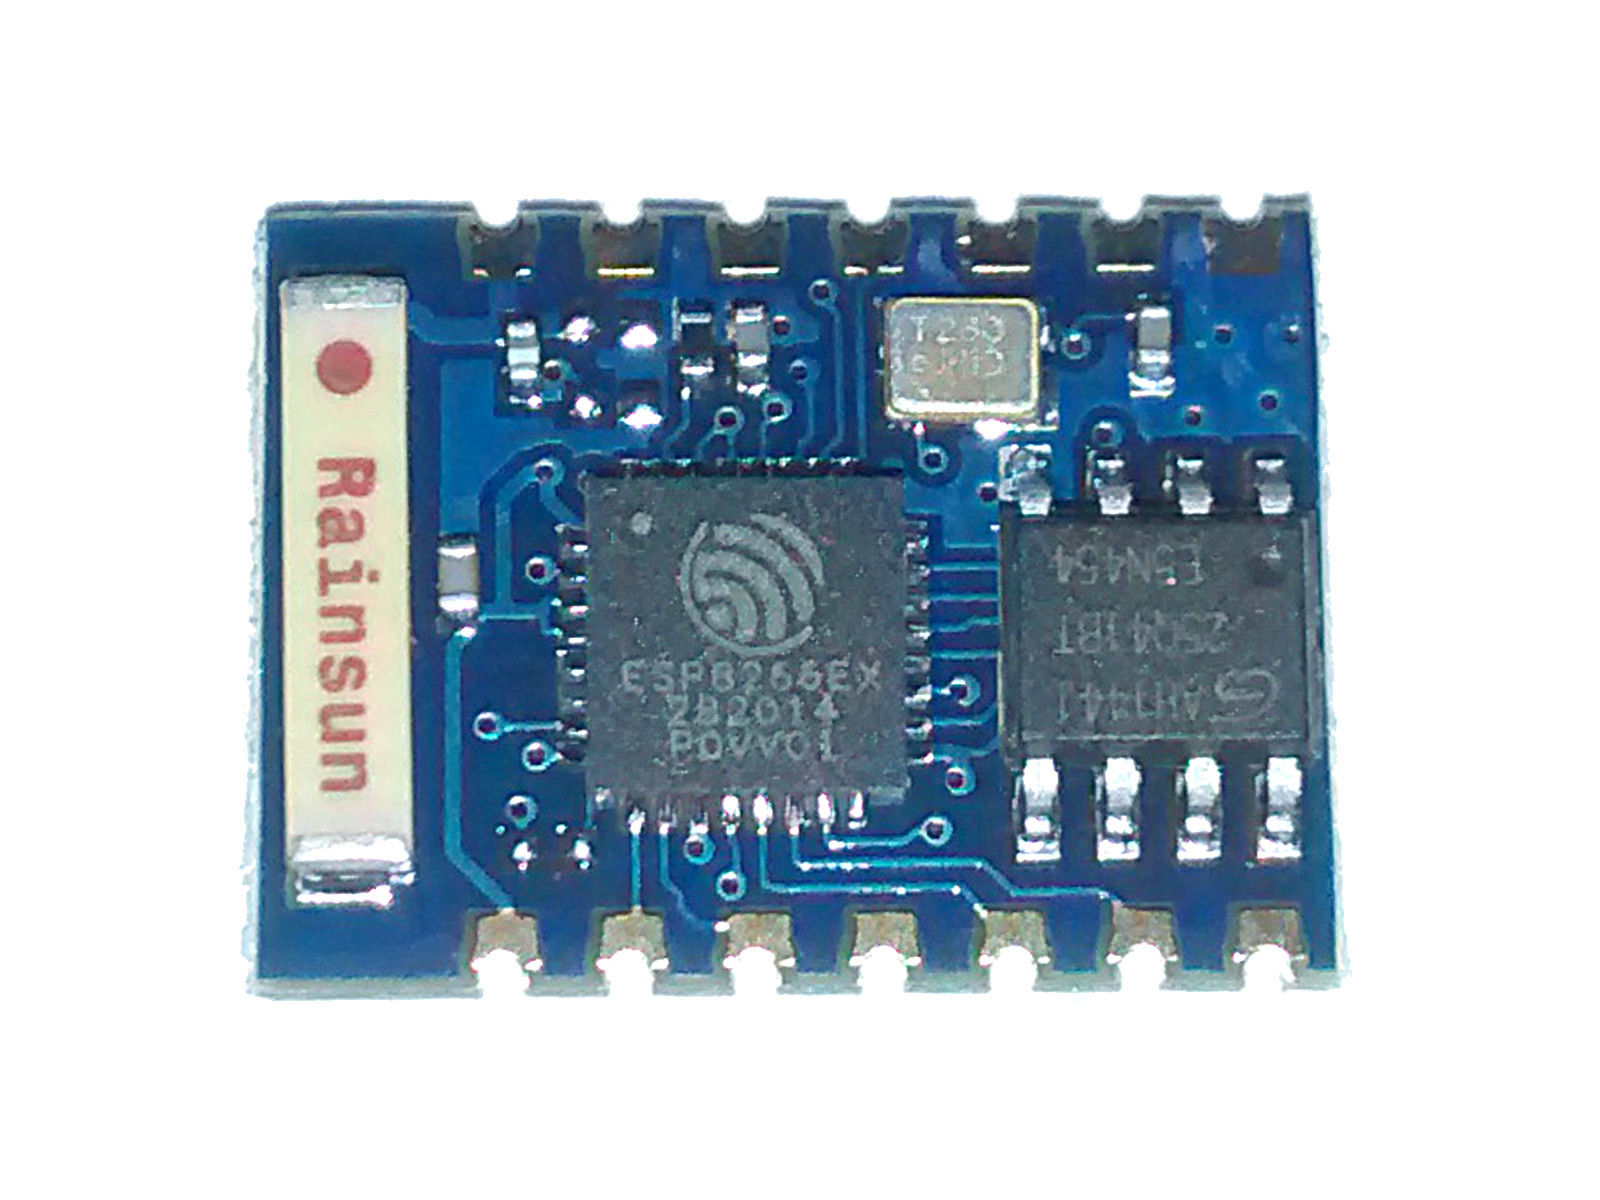
\includegraphics[scale=0.20]{ESP-01}
	\caption{ESP8266-01 module. You can see that distance between each pin is small which meant for us that it was hard to sold for someone inexperienced}
	\label{fig:ESP}
\end{figure}

\chapter{Latex Listings}
The code highlighting in this tex document was taken from \href{https://github.com/trihedral/ArduinoLatexListing/blob/master/arduinoLanguage.tex}{trihedral's ArduinoLatexListing Github repository}


\begin{lstlisting}[caption={models}\label{list:Models}, language=CSharp]
public class ArduinoData
{
	public int Temperature { get; set; }
	public uint Moisture { get; set; }
	public Plant Plant { get; set; }
	public uint PlantId { get; set; }
	[Key]
    public long DataId { get; set; }
	public int Light { get;  set; }
	public int Water { get;  set; }
}

public class Plant
{
	public long PlantId { get; set; }
    public string Name { get; set; }
	public DateTime DateAdded { get; set; }
	public ApplicationUser ApplicationUser { get; set; }
	public IList<ArduinoData> Datas { get; set; }
}

public class ApplicationUser : IdentityUser
{
	public string Name { get; set; }
	public virtual List<Plant> Plants { get; set; }  
}
\end{lstlisting}

\begin{lstlisting}[caption={ArduinoDataRepository}\label{list:Observer},language=CSharp]
public interface IArduinoDataRepository
{
	void SaveData(ArduinoData data);
}

public interface IPlantRepository
{
	Task<IEnumerable<Plant>> UserPlants();
    Task SavePlant(Plant plant);
} 

public interface IUserRepository
{
	ApplicationUser GetCurrentUser();
}

\end{lstlisting}

\begin{lstlisting}[caption={Observer Class}\label{list:Observer}, language=CSharp]
public class Observer : IObserver<ArduinoData>
{
	private IDisposable _unsubscriber;
    public EFArduinoDataRepository ArduinoDataRepository { get; set; }

      
	public void Subscribe(IObservable<ArduinoData> provider)
    {
		if (provider != null)
        _unsubscriber = provider.Subscribe(this);
	}

	public virtual void OnCompleted()
	{
	Console.WriteLine($"connection to observer closed.");
	this.Unsubscribe();
	}

	public virtual void OnError(Exception e)
	{
	Console.WriteLine($"Observer: Error in connection or transmission of data.");
	}

	// This runs when data from arduino is received.
	public virtual void OnNext(ArduinoData value)
	{
		ArduinoDataRepository.SaveData(value); // save the read data 							                           		//into the data repository 
	}

	public virtual void Unsubscribe()
	{
		_unsubscriber.Dispose();
	}
}
\end{lstlisting}

\backmatter 
\cleardoublepage\addcontentsline{toc}{chapter}{Bibliography}
\bibliographystyle{plain}
\bibliography{bibliography}
\end{document}
